% Created by tikzDevice version 0.12 on 2019-06-12 00:00:38
% !TEX encoding = UTF-8 Unicode
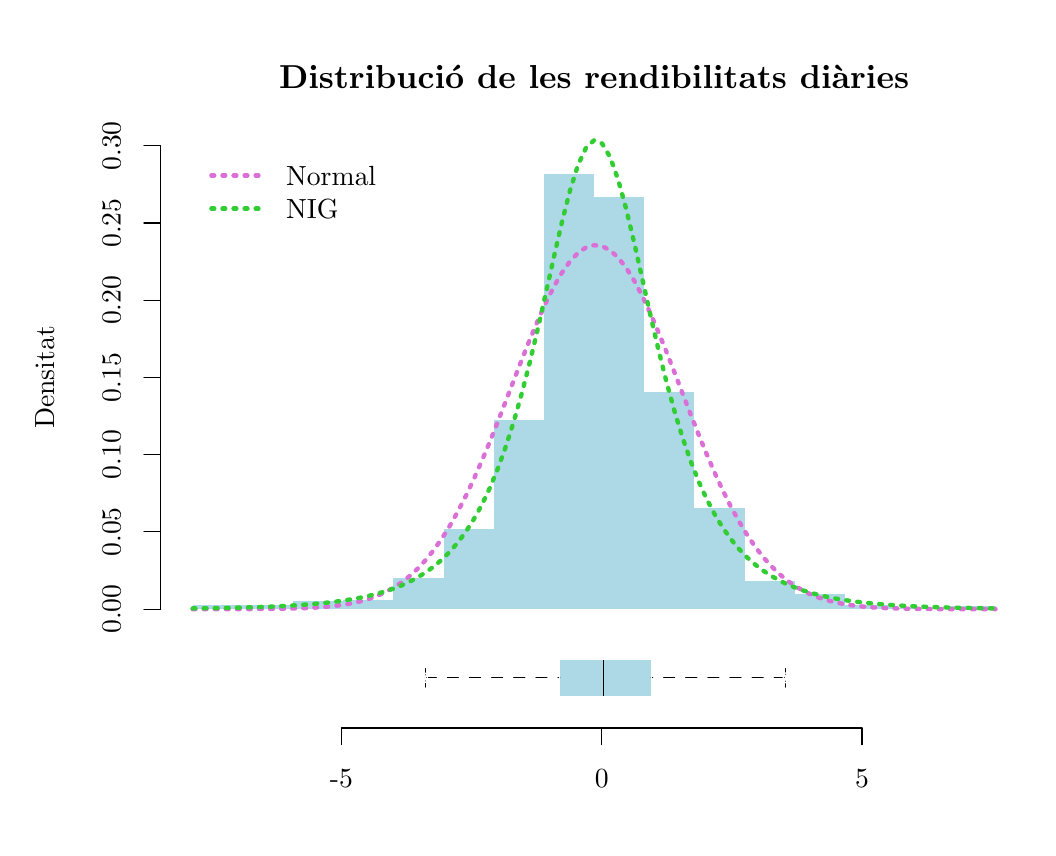
\begin{tikzpicture}[x=1pt,y=1pt]
\definecolor{fillColor}{RGB}{255,255,255}
\path[use as bounding box,fill=fillColor,fill opacity=0.00] (0,0) rectangle (361.35,289.08);
\begin{scope}
\path[clip] ( 48.00, 36.00) rectangle (361.35, 72.27);
\definecolor{fillColor}{RGB}{173,216,230}

\path[fill=fillColor] (192.30, 47.42) --
	(192.30, 60.85) --
	(225.26, 60.85) --
	(225.26, 47.42) --
	cycle;
\definecolor{drawColor}{RGB}{0,0,0}

\path[draw=drawColor,line width= 0.4pt,line join=round] (207.93, 47.42) -- (207.93, 60.85);

\path[draw=drawColor,line width= 0.4pt,dash pattern=on 4pt off 4pt ,line join=round,line cap=round] (143.64, 54.14) -- (192.30, 54.14);

\path[draw=drawColor,line width= 0.4pt,dash pattern=on 4pt off 4pt ,line join=round,line cap=round] (273.78, 54.14) -- (225.26, 54.14);

\path[draw=drawColor,line width= 0.4pt,line join=round,line cap=round] (143.64, 50.78) -- (143.64, 57.49);

\path[draw=drawColor,line width= 0.4pt,line join=round,line cap=round] (273.78, 50.78) -- (273.78, 57.49);
\definecolor{drawColor}{RGB}{255,255,255}

\path[draw=drawColor,line width= 0.4pt,line join=round,line cap=round] (192.30, 47.42) --
	(192.30, 60.85) --
	(225.26, 60.85) --
	(225.26, 47.42) --
	(192.30, 47.42);

\path[draw=drawColor,line width= 0.4pt,line join=round,line cap=round] (105.45, 54.14) circle (  2.25);

\path[draw=drawColor,line width= 0.4pt,line join=round,line cap=round] ( 67.24, 54.14) circle (  2.25);

\path[draw=drawColor,line width= 0.4pt,line join=round,line cap=round] (277.76, 54.14) circle (  2.25);

\path[draw=drawColor,line width= 0.4pt,line join=round,line cap=round] (275.24, 54.14) circle (  2.25);

\path[draw=drawColor,line width= 0.4pt,line join=round,line cap=round] (138.27, 54.14) circle (  2.25);

\path[draw=drawColor,line width= 0.4pt,line join=round,line cap=round] (276.00, 54.14) circle (  2.25);

\path[draw=drawColor,line width= 0.4pt,line join=round,line cap=round] ( 85.71, 54.14) circle (  2.25);

\path[draw=drawColor,line width= 0.4pt,line join=round,line cap=round] (304.50, 54.14) circle (  2.25);

\path[draw=drawColor,line width= 0.4pt,line join=round,line cap=round] (120.46, 54.14) circle (  2.25);

\path[draw=drawColor,line width= 0.4pt,line join=round,line cap=round] (127.44, 54.14) circle (  2.25);

\path[draw=drawColor,line width= 0.4pt,line join=round,line cap=round] (296.66, 54.14) circle (  2.25);

\path[draw=drawColor,line width= 0.4pt,line join=round,line cap=round] (141.54, 54.14) circle (  2.25);

\path[draw=drawColor,line width= 0.4pt,line join=round,line cap=round] (133.52, 54.14) circle (  2.25);

\path[draw=drawColor,line width= 0.4pt,line join=round,line cap=round] (110.29, 54.14) circle (  2.25);

\path[draw=drawColor,line width= 0.4pt,line join=round,line cap=round] (294.39, 54.14) circle (  2.25);

\path[draw=drawColor,line width= 0.4pt,line join=round,line cap=round] (286.35, 54.14) circle (  2.25);

\path[draw=drawColor,line width= 0.4pt,line join=round,line cap=round] (285.74, 54.14) circle (  2.25);

\path[draw=drawColor,line width= 0.4pt,line join=round,line cap=round] (129.37, 54.14) circle (  2.25);

\path[draw=drawColor,line width= 0.4pt,line join=round,line cap=round] (280.86, 54.14) circle (  2.25);

\path[draw=drawColor,line width= 0.4pt,line join=round,line cap=round] (140.10, 54.14) circle (  2.25);

\path[draw=drawColor,line width= 0.4pt,line join=round,line cap=round] ( 78.32, 54.14) circle (  2.25);

\path[draw=drawColor,line width= 0.4pt,line join=round,line cap=round] (302.05, 54.14) circle (  2.25);

\path[draw=drawColor,line width= 0.4pt,line join=round,line cap=round] (289.79, 54.14) circle (  2.25);

\path[draw=drawColor,line width= 0.4pt,line join=round,line cap=round] (346.93, 54.14) circle (  2.25);

\path[draw=drawColor,line width= 0.4pt,line join=round,line cap=round] (125.16, 54.14) circle (  2.25);

\path[draw=drawColor,line width= 0.4pt,line join=round,line cap=round] (349.74, 54.14) circle (  2.25);

\path[draw=drawColor,line width= 0.4pt,line join=round,line cap=round] (314.87, 54.14) circle (  2.25);

\path[draw=drawColor,line width= 0.4pt,line join=round,line cap=round] (298.87, 54.14) circle (  2.25);

\path[draw=drawColor,line width= 0.4pt,line join=round,line cap=round] (129.29, 54.14) circle (  2.25);

\path[draw=drawColor,line width= 0.4pt,line join=round,line cap=round] (102.83, 54.14) circle (  2.25);

\path[draw=drawColor,line width= 0.4pt,line join=round,line cap=round] (128.48, 54.14) circle (  2.25);

\path[draw=drawColor,line width= 0.4pt,line join=round,line cap=round] ( 96.81, 54.14) circle (  2.25);

\path[draw=drawColor,line width= 0.4pt,line join=round,line cap=round] (141.02, 54.14) circle (  2.25);

\path[draw=drawColor,line width= 0.4pt,line join=round,line cap=round] ( 87.03, 54.14) circle (  2.25);

\path[draw=drawColor,line width= 0.4pt,line join=round,line cap=round] (138.12, 54.14) circle (  2.25);

\path[draw=drawColor,line width= 0.4pt,line join=round,line cap=round] (283.11, 54.14) circle (  2.25);

\path[draw=drawColor,line width= 0.4pt,line join=round,line cap=round] (137.35, 54.14) circle (  2.25);

\path[draw=drawColor,line width= 0.4pt,line join=round,line cap=round] (133.79, 54.14) circle (  2.25);

\path[draw=drawColor,line width= 0.4pt,line join=round,line cap=round] (132.24, 54.14) circle (  2.25);

\path[draw=drawColor,line width= 0.4pt,line join=round,line cap=round] ( 59.61, 54.14) circle (  2.25);

\path[draw=drawColor,line width= 0.4pt,line join=round,line cap=round] ( 99.44, 54.14) circle (  2.25);

\path[draw=drawColor,line width= 0.4pt,line join=round,line cap=round] (289.52, 54.14) circle (  2.25);

\path[draw=drawColor,line width= 0.4pt,line join=round,line cap=round] (142.19, 54.14) circle (  2.25);

\path[draw=drawColor,line width= 0.4pt,line join=round,line cap=round] (298.33, 54.14) circle (  2.25);

\path[draw=drawColor,line width= 0.4pt,line join=round,line cap=round] (284.40, 54.14) circle (  2.25);

\path[draw=drawColor,line width= 0.4pt,line join=round,line cap=round] ( 72.36, 54.14) circle (  2.25);

\path[draw=drawColor,line width= 0.4pt,line join=round,line cap=round] (135.46, 54.14) circle (  2.25);

\path[draw=drawColor,line width= 0.4pt,line join=round,line cap=round] (329.01, 54.14) circle (  2.25);
\end{scope}
\begin{scope}
\path[clip] (  0.00,  0.00) rectangle (361.35,289.08);
\definecolor{drawColor}{RGB}{0,0,0}

\path[draw=drawColor,line width= 0.4pt,line join=round,line cap=round] (113.40, 36.00) -- (301.47, 36.00);

\path[draw=drawColor,line width= 0.4pt,line join=round,line cap=round] (113.40, 36.00) -- (113.40, 30.00);

\path[draw=drawColor,line width= 0.4pt,line join=round,line cap=round] (207.44, 36.00) -- (207.44, 30.00);

\path[draw=drawColor,line width= 0.4pt,line join=round,line cap=round] (301.47, 36.00) -- (301.47, 30.00);

\node[text=drawColor,anchor=base,inner sep=0pt, outer sep=0pt, scale=  1.00] at (113.40, 14.40) {-5};

\node[text=drawColor,anchor=base,inner sep=0pt, outer sep=0pt, scale=  1.00] at (207.44, 14.40) {0};

\node[text=drawColor,anchor=base,inner sep=0pt, outer sep=0pt, scale=  1.00] at (301.47, 14.40) {5};
\end{scope}
\begin{scope}
\path[clip] (  0.00, 72.27) rectangle (361.35,289.08);
\definecolor{drawColor}{RGB}{0,0,0}

\node[text=drawColor,anchor=base,inner sep=0pt, outer sep=0pt, scale=  1.20] at (204.67,266.94) {\bfseries Distribució de les rendibilitats diàries};

\node[text=drawColor,rotate= 90.00,anchor=base,inner sep=0pt, outer sep=0pt, scale=  1.00] at (  9.60,162.68) {Densitat};
\end{scope}
\begin{scope}
\path[clip] (  0.00,  0.00) rectangle (361.35,289.08);
\definecolor{drawColor}{RGB}{0,0,0}

\path[draw=drawColor,line width= 0.4pt,line join=round,line cap=round] ( 48.00, 78.97) -- ( 48.00,246.38);

\path[draw=drawColor,line width= 0.4pt,line join=round,line cap=round] ( 48.00, 78.97) -- ( 42.00, 78.97);

\path[draw=drawColor,line width= 0.4pt,line join=round,line cap=round] ( 48.00,106.87) -- ( 42.00,106.87);

\path[draw=drawColor,line width= 0.4pt,line join=round,line cap=round] ( 48.00,134.77) -- ( 42.00,134.77);

\path[draw=drawColor,line width= 0.4pt,line join=round,line cap=round] ( 48.00,162.68) -- ( 42.00,162.68);

\path[draw=drawColor,line width= 0.4pt,line join=round,line cap=round] ( 48.00,190.58) -- ( 42.00,190.58);

\path[draw=drawColor,line width= 0.4pt,line join=round,line cap=round] ( 48.00,218.48) -- ( 42.00,218.48);

\path[draw=drawColor,line width= 0.4pt,line join=round,line cap=round] ( 48.00,246.38) -- ( 42.00,246.38);

\node[text=drawColor,rotate= 90.00,anchor=base,inner sep=0pt, outer sep=0pt, scale=  1.00] at ( 33.60, 78.97) {0.00};

\node[text=drawColor,rotate= 90.00,anchor=base,inner sep=0pt, outer sep=0pt, scale=  1.00] at ( 33.60,106.87) {0.05};

\node[text=drawColor,rotate= 90.00,anchor=base,inner sep=0pt, outer sep=0pt, scale=  1.00] at ( 33.60,134.77) {0.10};

\node[text=drawColor,rotate= 90.00,anchor=base,inner sep=0pt, outer sep=0pt, scale=  1.00] at ( 33.60,162.68) {0.15};

\node[text=drawColor,rotate= 90.00,anchor=base,inner sep=0pt, outer sep=0pt, scale=  1.00] at ( 33.60,190.58) {0.20};

\node[text=drawColor,rotate= 90.00,anchor=base,inner sep=0pt, outer sep=0pt, scale=  1.00] at ( 33.60,218.48) {0.25};

\node[text=drawColor,rotate= 90.00,anchor=base,inner sep=0pt, outer sep=0pt, scale=  1.00] at ( 33.60,246.38) {0.30};
\end{scope}
\begin{scope}
\path[clip] ( 48.00, 72.27) rectangle (361.35,253.08);
\definecolor{fillColor}{RGB}{173,216,230}

\path[fill=fillColor] ( 59.61, 78.97) rectangle ( 77.74, 80.63);

\path[fill=fillColor] ( 77.74, 78.97) rectangle ( 95.87, 80.63);

\path[fill=fillColor] ( 95.87, 78.97) rectangle (114.01, 81.75);

\path[fill=fillColor] (114.01, 78.97) rectangle (132.14, 82.30);

\path[fill=fillColor] (132.14, 78.97) rectangle (150.27, 90.08);

\path[fill=fillColor] (150.27, 78.97) rectangle (168.41,107.87);

\path[fill=fillColor] (168.41, 78.97) rectangle (186.54,147.33);

\path[fill=fillColor] (186.54, 78.97) rectangle (204.67,236.27);

\path[fill=fillColor] (204.67, 78.97) rectangle (222.81,227.93);

\path[fill=fillColor] (222.81, 78.97) rectangle (240.94,157.34);

\path[fill=fillColor] (240.94, 78.97) rectangle (259.08,115.65);

\path[fill=fillColor] (259.08, 78.97) rectangle (277.21, 88.97);

\path[fill=fillColor] (277.21, 78.97) rectangle (295.34, 84.52);

\path[fill=fillColor] (295.34, 78.97) rectangle (313.48, 80.63);

\path[fill=fillColor] (313.48, 78.97) rectangle (331.61, 79.52);

\path[fill=fillColor] (331.61, 78.97) rectangle (349.74, 80.08);
\definecolor{drawColor}{RGB}{218,112,214}

\path[draw=drawColor,line width= 1.6pt,dash pattern=on 1pt off 3pt ,line join=round,line cap=round] ( 59.61, 78.97) --
	( 62.51, 78.97) --
	( 65.41, 78.97) --
	( 68.31, 78.97) --
	( 71.21, 78.98) --
	( 74.11, 78.98) --
	( 77.01, 78.99) --
	( 79.92, 79.00) --
	( 82.82, 79.01) --
	( 85.72, 79.03) --
	( 88.62, 79.06) --
	( 91.52, 79.10) --
	( 94.42, 79.16) --
	( 97.32, 79.24) --
	(100.23, 79.34) --
	(103.13, 79.49) --
	(106.03, 79.67) --
	(108.93, 79.92) --
	(111.83, 80.25) --
	(114.73, 80.67) --
	(117.63, 81.20) --
	(120.53, 81.88) --
	(123.44, 82.74) --
	(126.34, 83.80) --
	(129.24, 85.10) --
	(132.14, 86.68) --
	(135.04, 88.58) --
	(137.94, 90.85) --
	(140.84, 93.52) --
	(143.75, 96.64) --
	(146.65,100.23) --
	(149.55,104.32) --
	(152.45,108.93) --
	(155.35,114.07) --
	(158.25,119.71) --
	(161.15,125.85) --
	(164.06,132.43) --
	(166.96,139.39) --
	(169.86,146.65) --
	(172.76,154.11) --
	(175.66,161.64) --
	(178.56,169.12) --
	(181.46,176.41) --
	(184.37,183.34) --
	(187.27,189.78) --
	(190.17,195.57) --
	(193.07,200.56) --
	(195.97,204.64) --
	(198.87,207.71) --
	(201.77,209.67) --
	(204.67,210.48) --
	(207.58,210.13) --
	(210.48,208.61) --
	(213.38,205.96) --
	(216.28,202.27) --
	(219.18,197.61) --
	(222.08,192.12) --
	(224.98,185.92) --
	(227.89,179.16) --
	(230.79,171.99) --
	(233.69,164.57) --
	(236.59,157.04) --
	(239.49,149.53) --
	(242.39,142.19) --
	(245.29,135.10) --
	(248.20,128.36) --
	(251.10,122.05) --
	(254.00,116.21) --
	(256.90,110.87) --
	(259.80,106.05) --
	(262.70,101.76) --
	(265.60, 97.98) --
	(268.51, 94.68) --
	(271.41, 91.84) --
	(274.31, 89.42) --
	(277.21, 87.38) --
	(280.11, 85.68) --
	(283.01, 84.27) --
	(285.91, 83.12) --
	(288.82, 82.19) --
	(291.72, 81.45) --
	(294.62, 80.86) --
	(297.52, 80.40) --
	(300.42, 80.04) --
	(303.32, 79.76) --
	(306.22, 79.55) --
	(309.12, 79.39) --
	(312.03, 79.28) --
	(314.93, 79.19) --
	(317.83, 79.12) --
	(320.73, 79.08) --
	(323.63, 79.04) --
	(326.53, 79.02) --
	(329.43, 79.00) --
	(332.34, 78.99) --
	(335.24, 78.98) --
	(338.14, 78.98) --
	(341.04, 78.97) --
	(343.94, 78.97) --
	(346.84, 78.97) --
	(349.74, 78.97);
\definecolor{drawColor}{RGB}{50,205,50}

\path[draw=drawColor,line width= 1.6pt,dash pattern=on 1pt off 3pt ,line join=round,line cap=round] ( 59.61, 79.23) --
	( 62.51, 79.27) --
	( 65.41, 79.31) --
	( 68.31, 79.35) --
	( 71.21, 79.41) --
	( 74.11, 79.47) --
	( 77.01, 79.54) --
	( 79.92, 79.61) --
	( 82.82, 79.70) --
	( 85.72, 79.80) --
	( 88.62, 79.92) --
	( 91.52, 80.06) --
	( 94.42, 80.21) --
	( 97.32, 80.38) --
	(100.23, 80.59) --
	(103.13, 80.82) --
	(106.03, 81.09) --
	(108.93, 81.39) --
	(111.83, 81.75) --
	(114.73, 82.16) --
	(117.63, 82.63) --
	(120.53, 83.17) --
	(123.44, 83.81) --
	(126.34, 84.54) --
	(129.24, 85.39) --
	(132.14, 86.37) --
	(135.04, 87.52) --
	(137.94, 88.85) --
	(140.84, 90.40) --
	(143.75, 92.20) --
	(146.65, 94.30) --
	(149.55, 96.75) --
	(152.45, 99.61) --
	(155.35,102.95) --
	(158.25,106.83) --
	(161.15,111.35) --
	(164.06,116.60) --
	(166.96,122.67) --
	(169.86,129.67) --
	(172.76,137.68) --
	(175.66,146.77) --
	(178.56,156.97) --
	(181.46,168.24) --
	(184.37,180.44) --
	(187.27,193.28) --
	(190.17,206.30) --
	(193.07,218.88) --
	(195.97,230.22) --
	(198.87,239.44) --
	(201.77,245.71) --
	(204.67,248.39) --
	(207.58,247.20) --
	(210.48,242.27) --
	(213.38,234.11) --
	(216.28,223.49) --
	(219.18,211.29) --
	(222.08,198.36) --
	(224.98,185.38) --
	(227.89,172.89) --
	(230.79,161.24) --
	(233.69,150.61) --
	(236.59,141.09) --
	(239.49,132.66) --
	(242.39,125.28) --
	(245.29,118.86) --
	(248.20,113.30) --
	(251.10,108.51) --
	(254.00,104.39) --
	(256.90,100.85) --
	(259.80, 97.82) --
	(262.70, 95.21) --
	(265.60, 92.98) --
	(268.51, 91.07) --
	(271.41, 89.42) --
	(274.31, 88.01) --
	(277.21, 86.80) --
	(280.11, 85.75) --
	(283.01, 84.85) --
	(285.91, 84.08) --
	(288.82, 83.41) --
	(291.72, 82.83) --
	(294.62, 82.33) --
	(297.52, 81.90) --
	(300.42, 81.53) --
	(303.32, 81.20) --
	(306.22, 80.92) --
	(309.12, 80.67) --
	(312.03, 80.46) --
	(314.93, 80.27) --
	(317.83, 80.11) --
	(320.73, 79.97) --
	(323.63, 79.85) --
	(326.53, 79.74) --
	(329.43, 79.65) --
	(332.34, 79.56) --
	(335.24, 79.49) --
	(338.14, 79.43) --
	(341.04, 79.37) --
	(343.94, 79.33) --
	(346.84, 79.28) --
	(349.74, 79.25);

\path[] ( 57.40,247.66) rectangle (130.42,211.66);
\definecolor{drawColor}{RGB}{218,112,214}

\path[draw=drawColor,line width= 1.6pt,dash pattern=on 1pt off 3pt ,line join=round,line cap=round] ( 66.40,235.66) -- ( 84.40,235.66);
\definecolor{drawColor}{RGB}{50,205,50}

\path[draw=drawColor,line width= 1.6pt,dash pattern=on 1pt off 3pt ,line join=round,line cap=round] ( 66.40,223.66) -- ( 84.40,223.66);
\definecolor{drawColor}{RGB}{0,0,0}

\node[text=drawColor,anchor=base west,inner sep=0pt, outer sep=0pt, scale=  1.00] at ( 93.40,232.21) {Normal};

\node[text=drawColor,anchor=base west,inner sep=0pt, outer sep=0pt, scale=  1.00] at ( 93.40,220.21) {NIG};
\end{scope}
\end{tikzpicture}
